% Editable native annotations around unchanged verified IDE photographs.
\par
\begin{figure}[htbp]
\centering
\newsavebox{\MARSchachastreamregistersBox}
\sbox{\MARSchachastreamregistersBox}{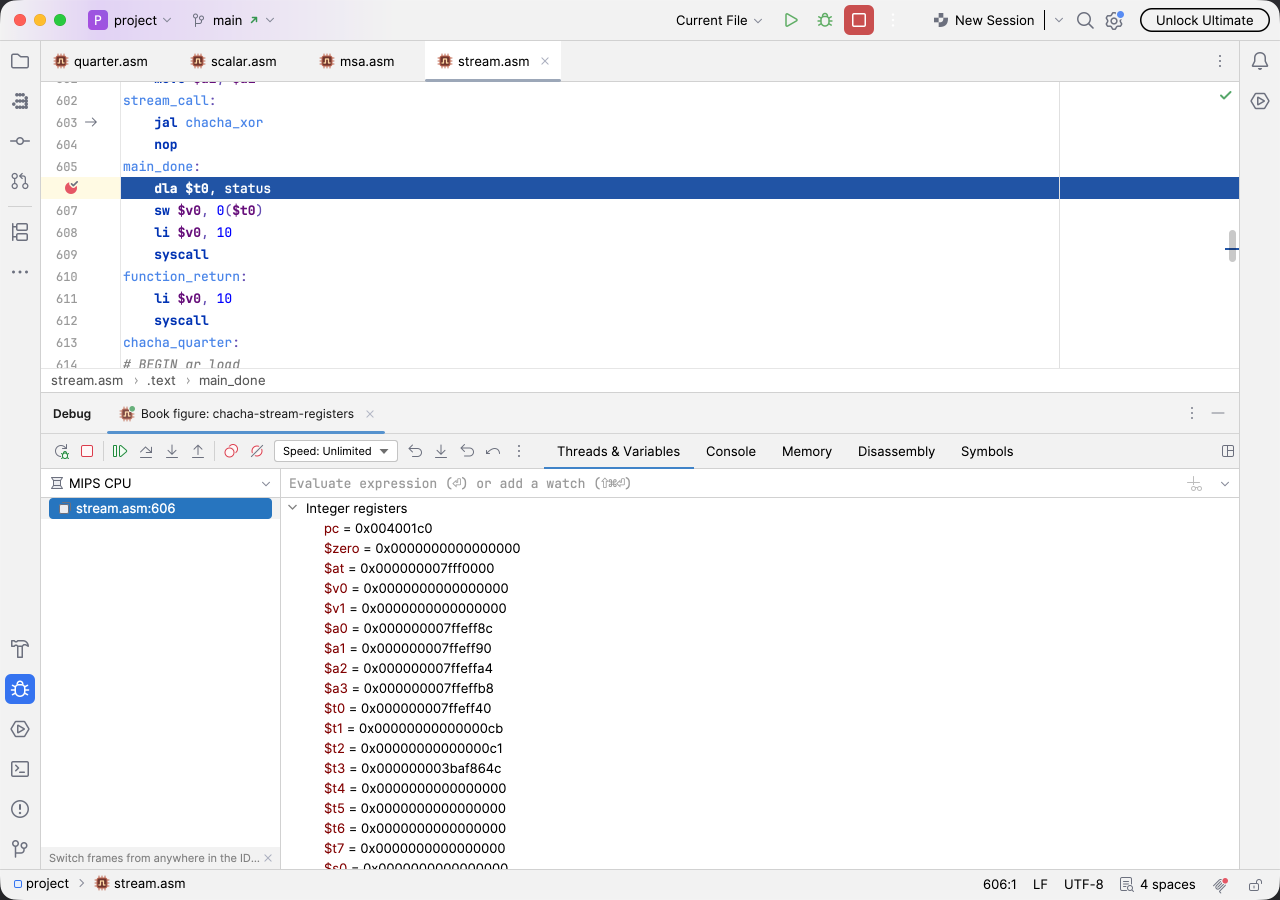
\includegraphics[artifact]{packages/026-chacha20/captures/f04/registers.png}}
\newsavebox{\MARSchachastreamoutputheadBox}
\sbox{\MARSchachastreamoutputheadBox}{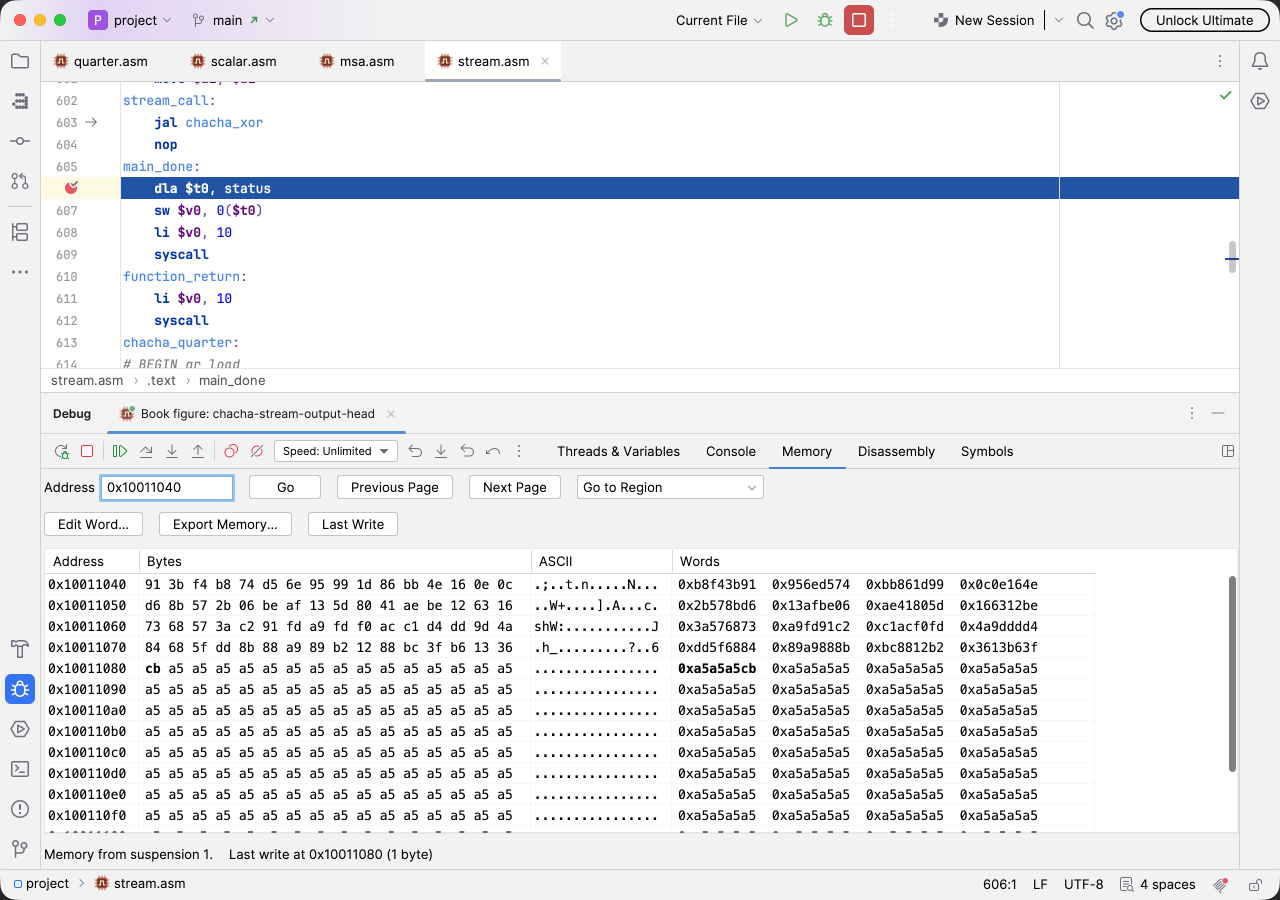
\includegraphics[artifact]{packages/026-chacha20/captures/f04/output-head.png}}
\newsavebox{\MARSchachastreamoutputtailBox}
\sbox{\MARSchachastreamoutputtailBox}{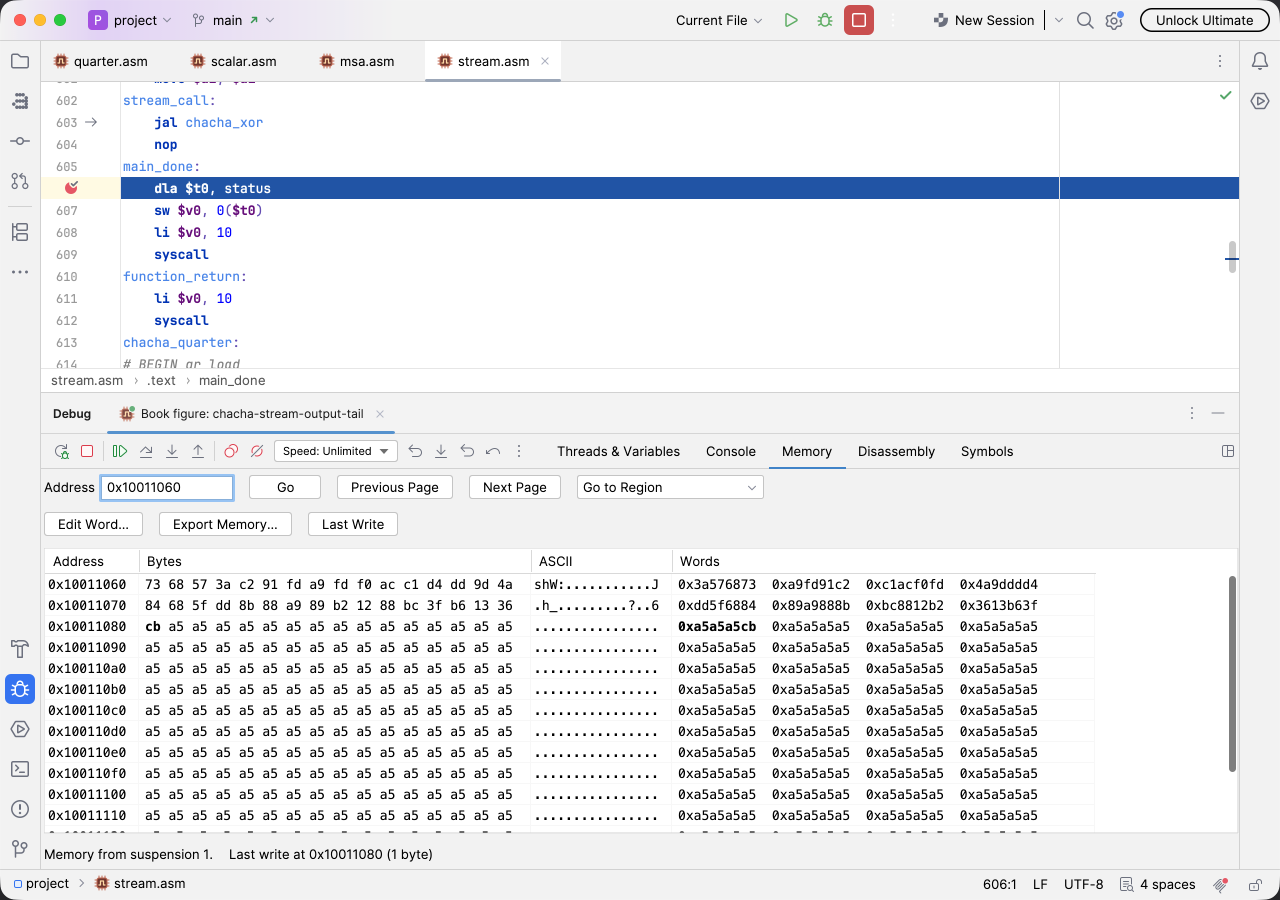
\includegraphics[artifact]{packages/026-chacha20/captures/f04/output-tail.png}}
\newsavebox{\MARSchachastreamcounternonceBox}
\sbox{\MARSchachastreamcounternonceBox}{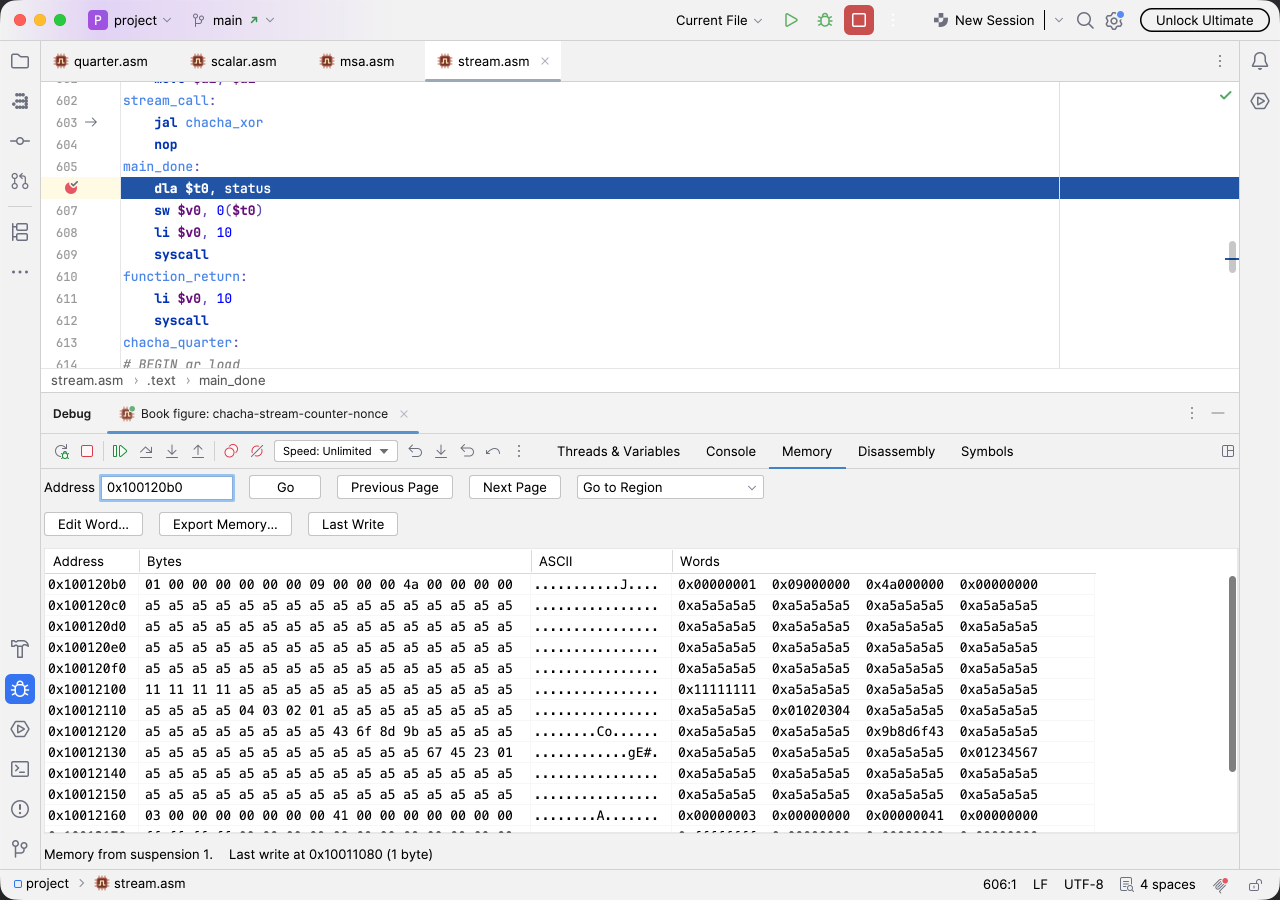
\includegraphics[artifact]{packages/026-chacha20/captures/f04/counter-nonce.png}}
\newsavebox{\MARSchachastreamsourceBox}
\sbox{\MARSchachastreamsourceBox}{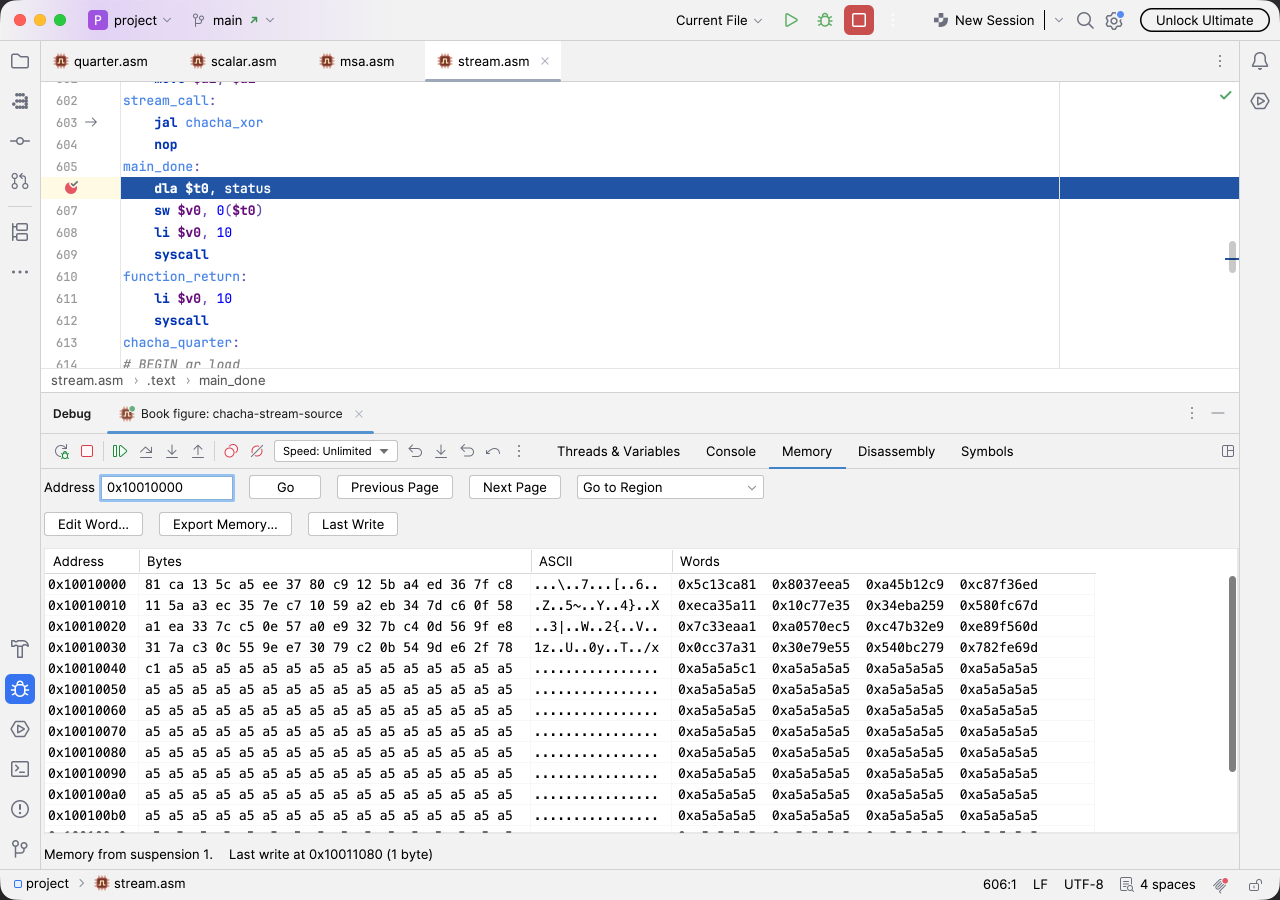
\includegraphics[artifact]{packages/026-chacha20/captures/f04/source.png}}
\edef\MARSchachastreamsourceLeft{\the\dimexpr0.036718750\wd\MARSchachastreamregistersBox\relax}
\edef\MARSchachastreamsourceBottom{\the\dimexpr0.774444444\ht\MARSchachastreamregistersBox\relax}
\edef\MARSchachastreamsourceRight{\the\dimexpr0.713281250\wd\MARSchachastreamregistersBox\relax}
\edef\MARSchachastreamsourceTop{\the\dimexpr0.170000000\ht\MARSchachastreamregistersBox\relax}
\edef\MARSchachastreamreturnsLeft{\the\dimexpr0.246093750\wd\MARSchachastreamregistersBox\relax}
\edef\MARSchachastreamreturnsBottom{\the\dimexpr0.334444444\ht\MARSchachastreamregistersBox\relax}
\edef\MARSchachastreamreturnsRight{\the\dimexpr0.553906250\wd\MARSchachastreamregistersBox\relax}
\edef\MARSchachastreamreturnsTop{\the\dimexpr0.640000000\ht\MARSchachastreamregistersBox\relax}
\edef\MARSchachastreamoutputheadLeft{\the\dimexpr0.034375000\wd\MARSchachastreamoutputheadBox\relax}
\edef\MARSchachastreamoutputheadBottom{\the\dimexpr0.311111111\ht\MARSchachastreamoutputheadBox\relax}
\edef\MARSchachastreamoutputheadRight{\the\dimexpr0.584375000\wd\MARSchachastreamoutputheadBox\relax}
\edef\MARSchachastreamoutputheadTop{\the\dimexpr0.608888889\ht\MARSchachastreamoutputheadBox\relax}
\edef\MARSchachastreamoutputtailLeft{\the\dimexpr0.034375000\wd\MARSchachastreamoutputtailBox\relax}
\edef\MARSchachastreamoutputtailBottom{\the\dimexpr0.287777778\ht\MARSchachastreamoutputtailBox\relax}
\edef\MARSchachastreamoutputtailRight{\the\dimexpr0.584375000\wd\MARSchachastreamoutputtailBox\relax}
\edef\MARSchachastreamoutputtailTop{\the\dimexpr0.608888889\ht\MARSchachastreamoutputtailBox\relax}
\edef\MARSchachastreamstateLeft{\the\dimexpr0.034375000\wd\MARSchachastreamcounternonceBox\relax}
\edef\MARSchachastreamstateBottom{\the\dimexpr0.334444444\ht\MARSchachastreamcounternonceBox\relax}
\edef\MARSchachastreamstateRight{\the\dimexpr0.584375000\wd\MARSchachastreamcounternonceBox\relax}
\edef\MARSchachastreamstateTop{\the\dimexpr0.608888889\ht\MARSchachastreamcounternonceBox\relax}
\edef\MARSchachastreaminputLeft{\the\dimexpr0.034375000\wd\MARSchachastreamsourceBox\relax}
\edef\MARSchachastreaminputBottom{\the\dimexpr0.311111111\ht\MARSchachastreamsourceBox\relax}
\edef\MARSchachastreaminputRight{\the\dimexpr0.584375000\wd\MARSchachastreamsourceBox\relax}
\edef\MARSchachastreaminputTop{\the\dimexpr0.608888889\ht\MARSchachastreamsourceBox\relax}
\begin{tikzpicture}[alt={Six annotated details at main_done show status zero, all sixty-five output bytes and the untouched destination suffix. The first sixty-four bytes use counter one and the last uses counter two. The original counter, nonce and input bytes remain unchanged; caller status has not yet been stored.}]
\node[anchor=north west,inner sep=0,font=\small\bfseries] (source-title) at (6mm,0) {Next caller instruction};
\node[anchor=north west,inner sep=0] (source) at ([yshift=-1mm]source-title.south west) {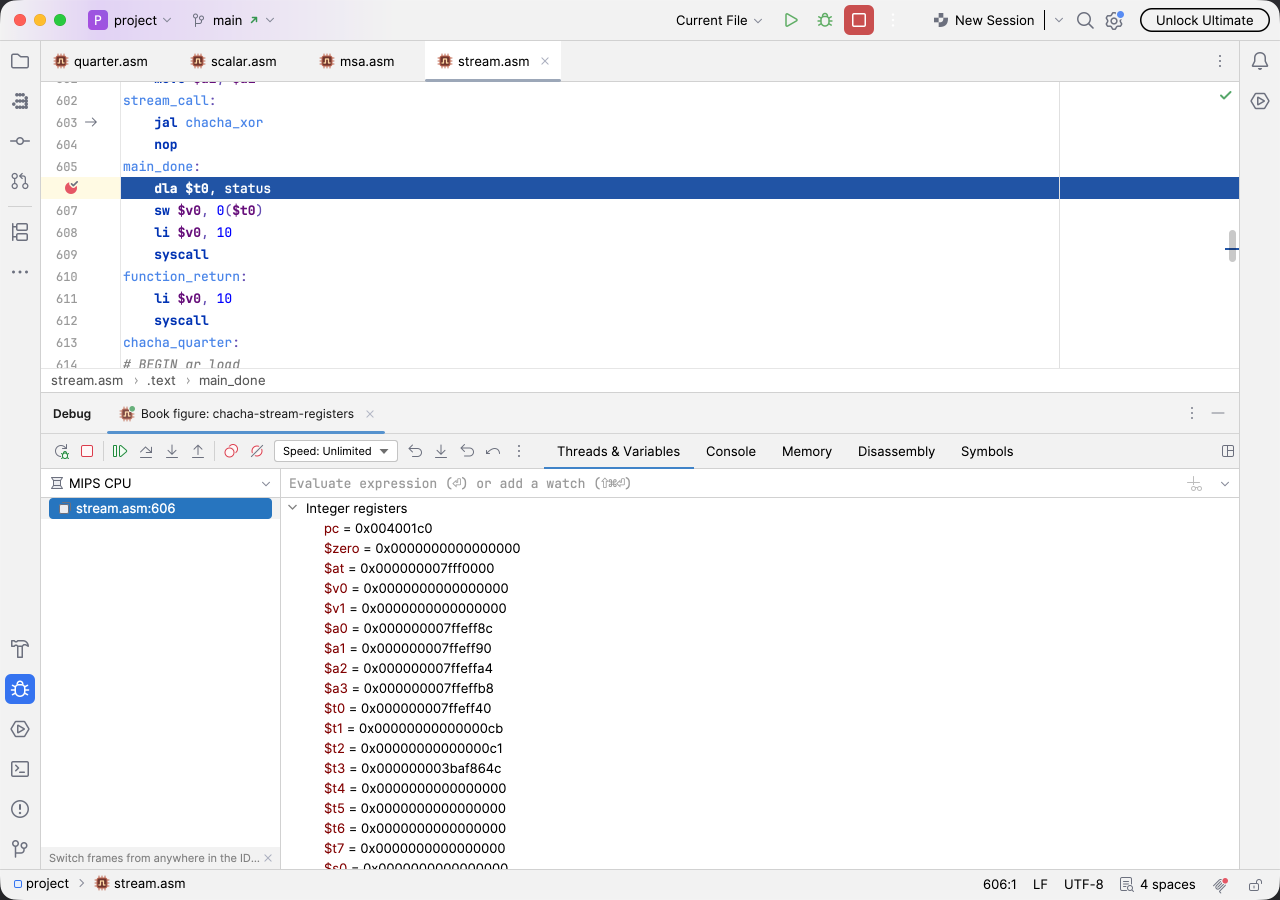
\includegraphics[width=0.50\linewidth,artifact,trim={\MARSchachastreamsourceLeft{} \MARSchachastreamsourceBottom{} \MARSchachastreamsourceRight{} \MARSchachastreamsourceTop{}},clip]{packages/026-chacha20/captures/f04/registers.png}};
\begin{scope}[shift={(source.south west)},x={($(source.south east)-(source.south west)$)},y={($(source.north west)-(source.south west)$)}]
\draw[black,line width=0.7pt] (0.237500000,0.080000000) rectangle (0.700000000,0.520000000);
\node[draw=black,fill=white,circle,inner sep=1.5pt,font=\footnotesize] at ($(0.237500000,0.520000000)+(-3mm,0)$) {1};
\end{scope}
\node[anchor=north west,inner sep=0,font=\small\bfseries] (returns-title) at (0.56\linewidth,0 |- source-title.north) {Successful return status};
\node[anchor=north west,inner sep=0] (returns) at ([yshift=-1mm]returns-title.south west) {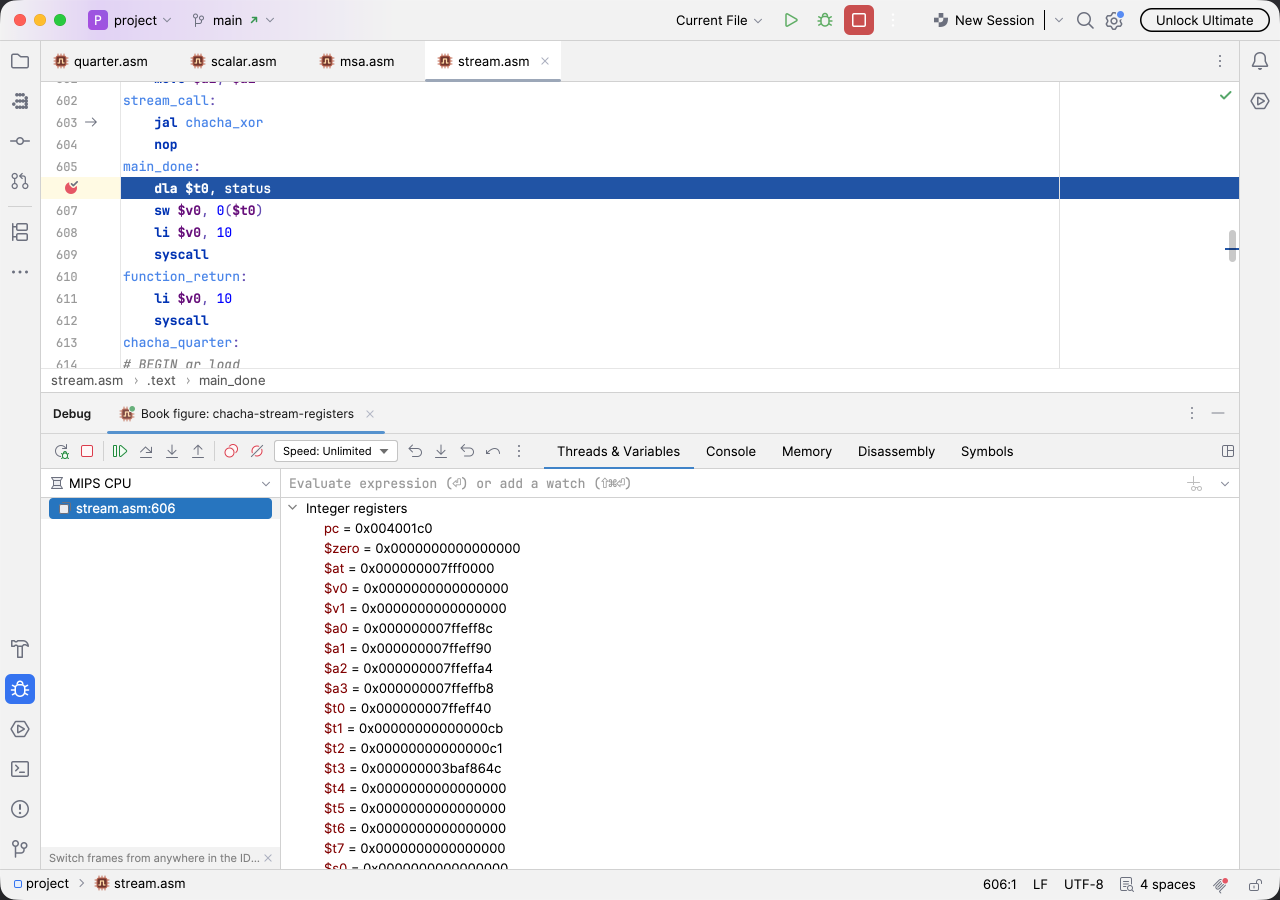
\includegraphics[width=0.42\linewidth,artifact,trim={\MARSchachastreamreturnsLeft{} \MARSchachastreamreturnsBottom{} \MARSchachastreamreturnsRight{} \MARSchachastreamreturnsTop{}},clip]{packages/026-chacha20/captures/f04/registers.png}};
\begin{scope}[shift={(returns.south west)},x={($(returns.south east)-(returns.south west)$)},y={($(returns.north west)-(returns.south west)$)}]
\draw[black,line width=0.7pt] (0.023437500,0.043478261) rectangle (0.761718750,0.913043478);
\node[draw=black,fill=white,circle,inner sep=1.5pt,font=\footnotesize] at ($(0.023437500,0.913043478)+(-3mm,0)$) {2};
\end{scope}
\node[anchor=north west,inner sep=0,font=\small\bfseries] (outputhead-title) at ([yshift=-1mm]source.south west) {Ciphertext bytes zero through thirty-one};
\node[anchor=north west,inner sep=0] (outputhead) at ([yshift=-1mm]outputhead-title.south west) {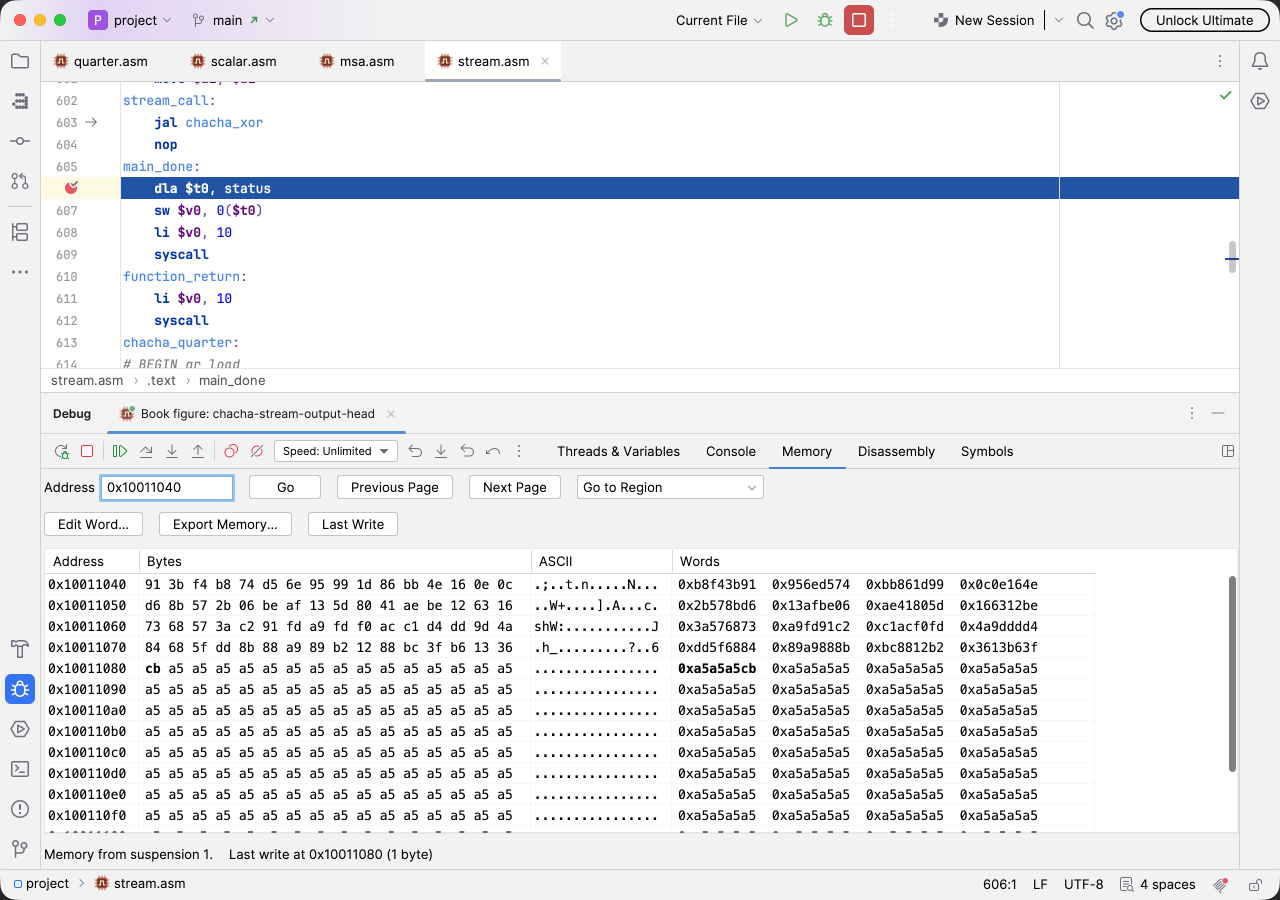
\includegraphics[width=0.84\linewidth,artifact,trim={\MARSchachastreamoutputheadLeft{} \MARSchachastreamoutputheadBottom{} \MARSchachastreamoutputheadRight{} \MARSchachastreamoutputheadTop{}},clip]{packages/026-chacha20/captures/f04/output-head.png}};
\begin{scope}[shift={(outputhead.south west)},x={($(outputhead.south east)-(outputhead.south west)$)},y={($(outputhead.north west)-(outputhead.south west)$)}]
\draw[black,line width=0.7pt] (0.194672131,0.055555556) rectangle (0.997950820,0.638888889);
\node[draw=black,fill=white,circle,inner sep=1.5pt,font=\footnotesize] at ($(0,0.638888889)+(-3mm,0)$) {3};
\end{scope}
\node[anchor=north west,inner sep=0,font=\small\bfseries] (outputtail-title) at ([yshift=-1mm]outputhead.south west) {Final ciphertext and untouched suffix};
\node[anchor=north west,inner sep=0] (outputtail) at ([yshift=-1mm]outputtail-title.south west) {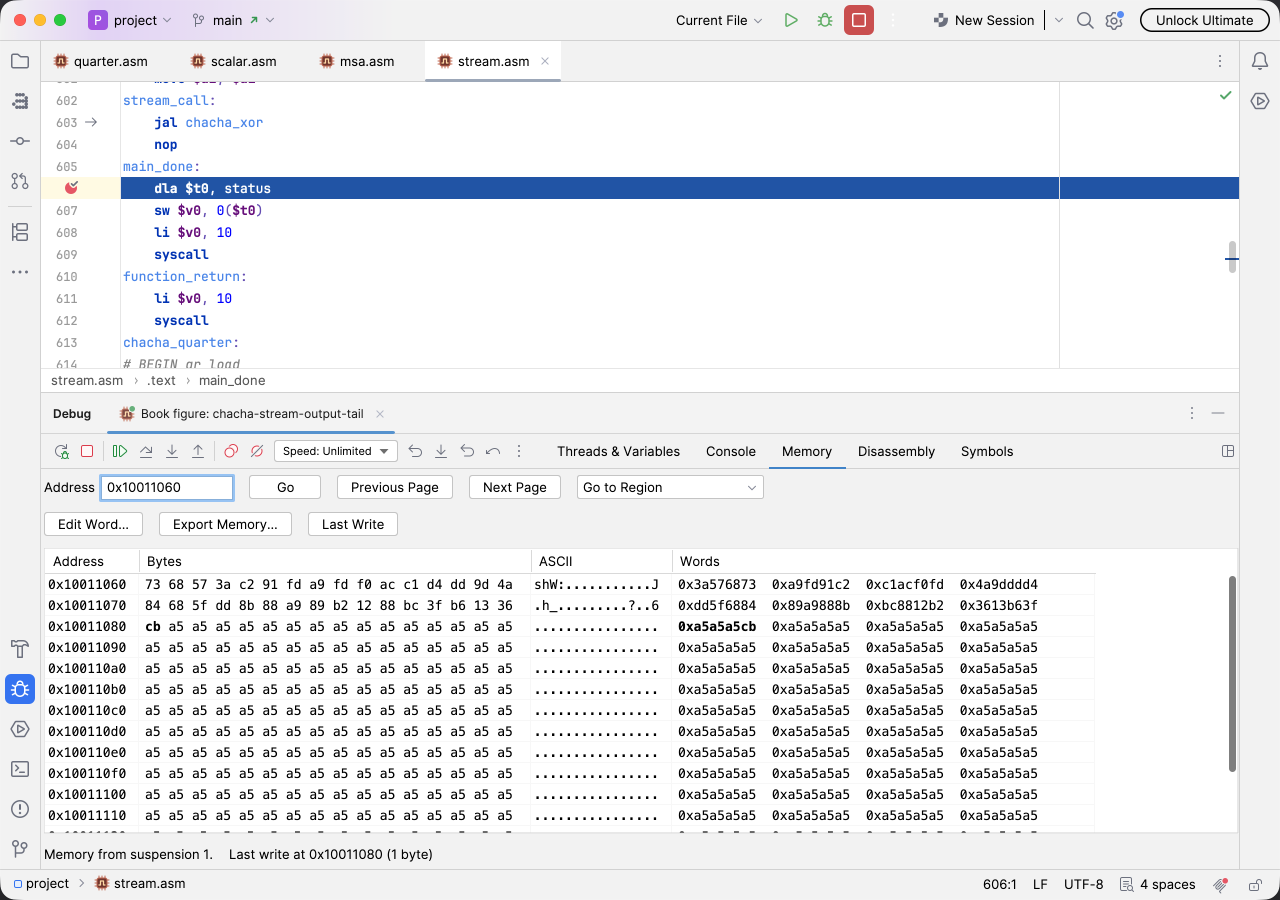
\includegraphics[width=0.84\linewidth,artifact,trim={\MARSchachastreamoutputtailLeft{} \MARSchachastreamoutputtailBottom{} \MARSchachastreamoutputtailRight{} \MARSchachastreamoutputtailTop{}},clip]{packages/026-chacha20/captures/f04/output-tail.png}};
\begin{scope}[shift={(outputtail.south west)},x={($(outputtail.south east)-(outputtail.south west)$)},y={($(outputtail.north west)-(outputtail.south west)$)}]
\draw[black,line width=0.7pt] (0.194672131,0.043010753) rectangle (0.997950820,0.720430108);
\node[draw=black,fill=white,circle,inner sep=1.5pt,font=\footnotesize] at ($(0,0.720430108)+(-3mm,0)$) {4};
\end{scope}
\node[anchor=north west,inner sep=0,font=\small\bfseries] (state-title) at ([yshift=-1mm]outputtail.south west) {Original counter and nonce};
\node[anchor=north west,inner sep=0] (state) at ([yshift=-1mm]state-title.south west) {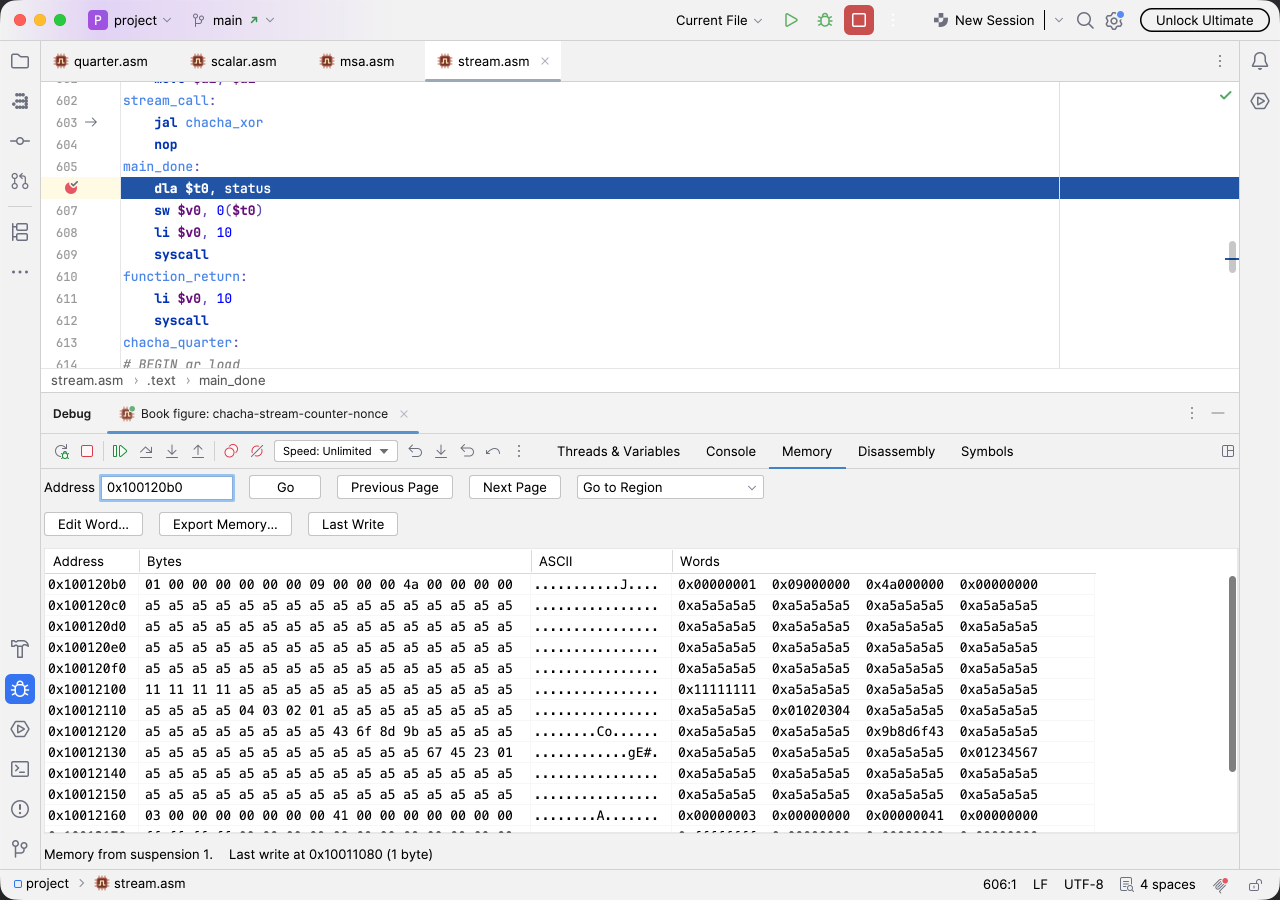
\includegraphics[width=0.84\linewidth,artifact,trim={\MARSchachastreamstateLeft{} \MARSchachastreamstateBottom{} \MARSchachastreamstateRight{} \MARSchachastreamstateTop{}},clip]{packages/026-chacha20/captures/f04/counter-nonce.png}};
\begin{scope}[shift={(state.south west)},x={($(state.south east)-(state.south west)$)},y={($(state.north west)-(state.south west)$)}]
\draw[black,line width=0.7pt] (0.194672131,0.078431373) rectangle (0.997950820,0.490196078);
\node[draw=black,fill=white,circle,inner sep=1.5pt,font=\footnotesize] at ($(0,0.490196078)+(-3mm,0)$) {5};
\end{scope}
\node[anchor=north west,inner sep=0,font=\small\bfseries] (input-title) at ([yshift=-1mm]state.south west) {Unchanged input prefix};
\node[anchor=north west,inner sep=0] (input) at ([yshift=-1mm]input-title.south west) {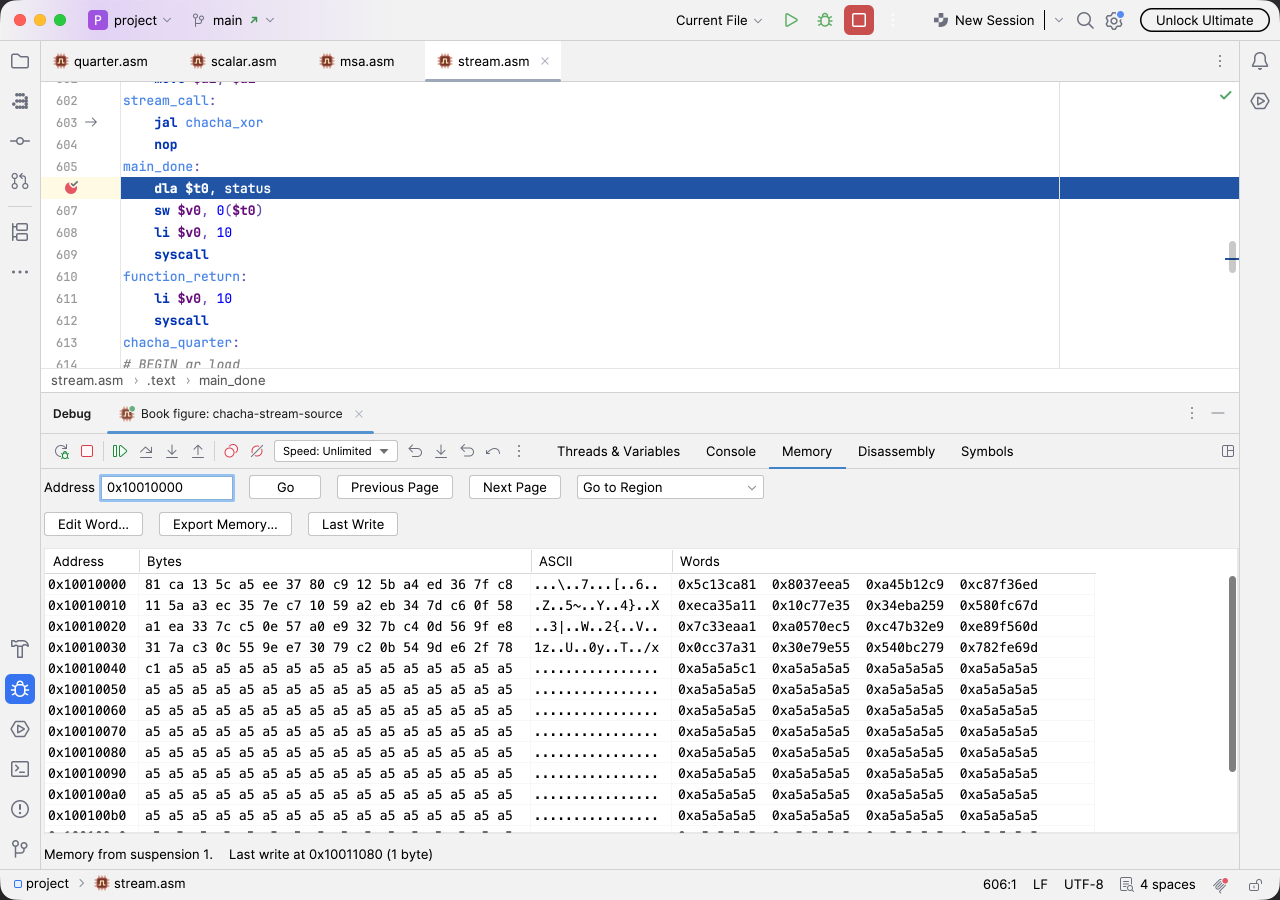
\includegraphics[width=0.84\linewidth,artifact,trim={\MARSchachastreaminputLeft{} \MARSchachastreaminputBottom{} \MARSchachastreaminputRight{} \MARSchachastreaminputTop{}},clip]{packages/026-chacha20/captures/f04/source.png}};
\begin{scope}[shift={(input.south west)},x={($(input.south east)-(input.south west)$)},y={($(input.north west)-(input.south west)$)}]
\draw[black,line width=0.7pt] (0.194672131,0.055555556) rectangle (0.997950820,0.638888889);
\node[draw=black,fill=white,circle,inner sep=1.5pt,font=\footnotesize] at ($(0,0.638888889)+(-3mm,0)$) {6};
\end{scope}
\end{tikzpicture}
\par\smallskip
\begin{minipage}{\linewidth}
\small
\begin{enumerate}
\setlength{\itemsep}{0pt}
\setlength{\parsep}{0pt}
\item The stop at \texttt{main\_done} follows the XOR routine return and precedes the caller status store. The routine has restored its frame and returned the output through memory.
\item \texttt{v0 = 0} reports success. The caller subsequently saves this status; this register does not contain ciphertext.
\item The first two output rows contain ciphertext bytes zero through thirty-one. Each is an input byte XORed with the corresponding serialized keystream byte.
\item The next two rows finish the first sixty-four-byte block. Only the first byte of the third row belongs to the message: byte sixty-four uses counter two. The following \texttt{a5} bytes remain untouched; no second full output block was written.
\item The caller state still contains counter one and the original nonce. Counter two was used only in a private stack copy. This whole-message interface does not return a retained partial-block streaming context.
\item The input prefix is unchanged because this recipe uses separate input and output. The independent check covers all input bytes, all sixty-five outputs, the destination suffix and the complete access history, including rejection of invisible same-value source stores.
\end{enumerate}
\end{minipage}
\caption{A sixty-five-byte message consumes one full block and one byte of the next.}
\label{capture:026-chacha20-f04}
\label{chacha-f04}
\end{figure}
\par
